\section{Prototipo}

\begin{figure}[ht!]
\begin{center}
	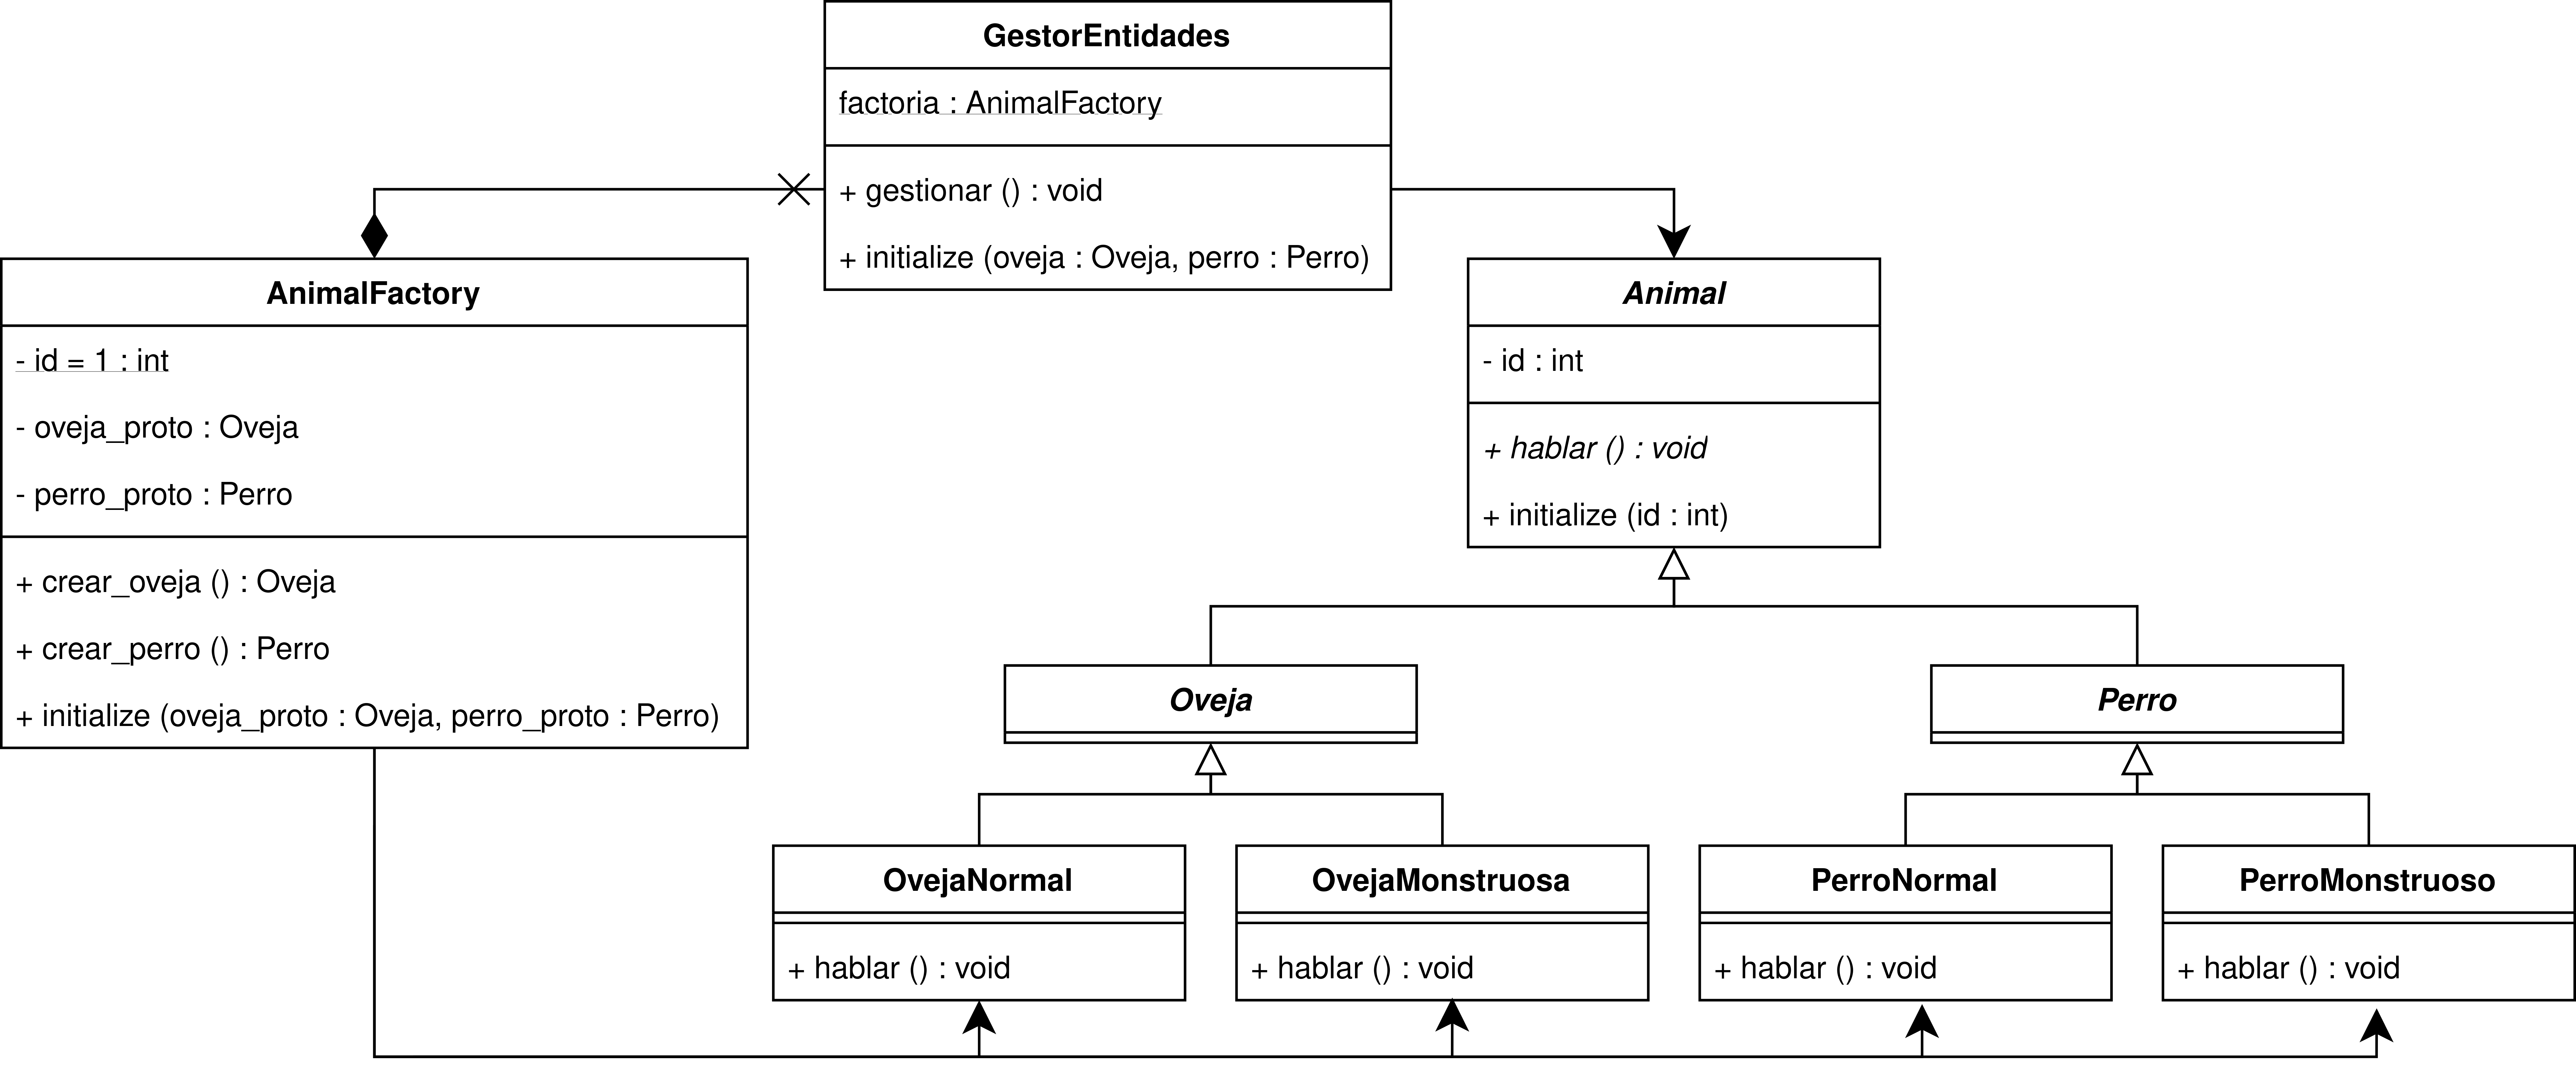
\includegraphics[scale=0.05]{DiagramaPrototipo}
\end{center}
\caption{Diagrama UML de la aplicación del patrón \textit{Prototipo}.}
\end{figure}

Nuestra aplicación del patrón \textit{Prototipo} consiste en una demo del sistema de creación de animales de \textit{CaveArt}.
Al inciar el programa, le preguntamos al jugador qué tipo de animales quiere y los almacenamos en \texttt{AnimalFactory} como prototipos.
Cuando esta clase crea los animales, llama al método \texttt{::clone} que tienen las clases por defecto en Ruby\footnote{%
	No hemos incluido \texttt{::clone} en el diagrama UML por no ser un método definido por nosotros.
}.

En la demostración puede verse fácilmente cómo cada animal se comporta de forma distinta en función de su naturaleza, imprimiendo un texto distinto en su método \texttt{::hablar}.
